\section{Additional notes on unsupervised sentiment analysis}
\label{sec:app_unsupervised_sentiment}

In this section we describe a model for inferring relationships between countries in an unsupervised fashion.  This model is based on the model in the last section, but it requires no explicit labels of the relationship between pairs of countries.  Instead it infers a qualitative relationship between countries -- a relationship which we can attempt to interpret post-hoc.  The significance of this approach is that it infers a relationship between countries based more on the discussion of these countries than explicit labels.  Particularly, if there is a relationship which has been overlooked by historians, then we might be able to learn it.

In the remainder of this section we will outline a probabilistic model
for inferring sentiment between pairs of countries.  We will outline
the key assumptions of this model -- first, a language model inspired
by the \emph{Networks Uncovered by Bayesian Inference} model
\citep{chang:2009nubbi}; and second, a spatial model of dyadic
relationships. We will then describe inference for this model, and
finally provide an empirical analysis of this model.

This section necessarily represents a very cursory look at
unsupervised sentiment analysis.  Because there are many parts to the
model, we focus on the \verb!intercept/distance! link function defined
in \mytab{fr_link_functions}.  As our goal is to qualitatively observe
the inferred sentiment topic, we will focus on that and skip a
rigorous analysis of this model's performance.

\subsection{A model of unsupervised foreign relations}

A key variable in this model is that each document has a sentiment parameter $\kappa_d$.  This become important when we link this sentiment model to text.  Intuitively, if two countries are far apart in the latent space at time $t$, we expect that $\kappa$ is more likely to be 1 when they interact.  Otherwise, $\kappa$ is more likely to be 0.  As we develop the language model, we will use this random variable to decide which topic is used to describe the pair of countries.

\subsubsection*{Binary Relational language model}
We incorporate text using a mixed-membership language model similar to
LDA.  Recall that in LDA, each word comes from a specific topic.  In
our model, which we dub the \emph{binary relational language model},
we assume that the words describing a pair of countries come from
topics about those countries.

\paragraph{A mixture of four topics.} To be concrete, consider a document discussing Iran and the United
States.  We assume that each word in this document will serve one of
four roles:
\begin{enumerate}
  \item It discusses the U.S. only,
  \item It discusses Iran only,
  \item It discusses the relationship between the U.S. and Iran. \label{foreign_relations:relationship}
  \item It is a ``filler'' word, providing little contribution to the discussion. \label{foreign_relations:filler}
\end{enumerate}
The first two roles for a word are self-explanatory.  The relationship in
(\ref{foreign_relations:relationship}) above could be any type of
relationship -- the goal of this section is of course to discover the
relationships in a collection of documents about these
countries.  The ``filler'' words in
(\ref{foreign_relations:filler}) above are those words found in any document
-- stopwords, for example -- that are unrelated to either country or
the relationship between them.

We therefore keep $(N_c + 2 + 1)$ topics---topics $\beta_{C,1},
\ldots, \beta_{C,{N_c}}$ for each of the $N_c$ countries, exactly two
sentiment topics $\beta_{S,0}, \beta_{S,1}$, and a single, global
background topic $\beta_{B0}$ \citep{chemudugunta:2009}.  We assume,
as in LDA, that a document about the United States and Iran is a
mixture of topics; in contrast to LDA, however, we constrain this
document's topics to be exactly the four topics enumerated above:
$\beta_{C,\mbox{\tiny Iran}}$, $\beta_{C,\mbox{\tiny United States}}$,
$\beta_{B,0}$, and either $\beta_{S,0}$ or $\beta_{S,1}$ (we describe
below how to make the choice between $\beta_{S,0}$ and $\beta_{S,1}$).
A document about Hungary and Germany, in contrast, would be a mixture
of the topics $\beta_{C,\mbox{\tiny Germany}}$, $\beta_{C,\mbox{\tiny
    Hungary}}$, $\beta_{B,0}$, and either $\beta_{S,0}$ or
$\beta_{S,1}$.

Once these topics are fixed for a document, the language model
proceeds as with LDA for each word: each word in the document comes
from one of four topics, with probability for topic $k$ proportional
to the topic mixture $\expect \theta_k$.  We illustrate this model
graphically in \myfig{binary_relational_language_model}.  Note that we
keep the topic mixture $\theta$ global instead of local to each
document because the topics are already very constrained.

\subsubsection{Determining the sentiment topic: connecting dyadic sentiment and text}

Up to now the dyadic sentiment model and the language model have been
developed independently.  We connect the two models by using the
binary sentiment parameter $\kappa_d$ to index the sentiment topic for
a document: document $d$ takes topic $\beta_{S,\kappa_d}$ for its
sentiment topic.\footnote{We also make a small adjustment to ensure
  that the model converges to a reasonable mode.  There are two main
  components of this model: a language model and a sentiment model. We
  introduce a parameter $\nu \sim \mathbb{N(0, 100)}$ and per-document
  parameters $\nu_d \sim \mathbb{R}(\nu, 0.001)$ and define the binary
  sentiment $\kappa_d \sim \sigma(s_d \nu_d)$.}
% determine the sentiment topic based on $k$.
In other words, if two countries are far apart in the latent space,
then when they interact in document $d$, this interaction is likely to
be negative (i.e., $\kappa_d = 1$, and the language used to describe
their relationship will come from topic $\beta_{S, 1}$.  If they were
instead close together in this latent space, the language used to
describe their relationship would come from topic $\beta_{S, 0}$.

We can now specify the generative model of a document language, given
the sentiment $\kappa_d$ for each interaction between countries.  We
begin by specifying the global topics.
\begin{enumerate}
\item First, draw topics:
  \begin{enumerate}
  \item For nation $c=1, \ldots, C$:
    \begin{itemize}
    \item Draw topic $\beta_{\mbox{C},c} \sim \mbox{Dir}(1, \ldots, 1)$.
    \end{itemize}
  \item Draw background topic $\beta_{\mbox{B},0} \sim \mbox{Dir}(1, \ldots, 1)$.
  \item Draw positive-interaction topic $\beta_{\mbox{S},0} \sim \mbox{Dir}(1, \ldots, 1)$
  \item Draw negative-interaction topic $\beta_{\mbox{S},1} \sim \mbox{Dir}(1, \ldots, 1)$
\end{enumerate}

\item Next, draw the global topic mixture $\theta \sim \mbox{Dir}(1, 1, 1, 1)$.

\item Finally, draw documents. \\
For document $d=1, \ldots, D$, each representing interactions between pairs of countries $c_{d,1},c_{d,2}$:
  \begin{enumerate}
    \item Draw sentiment index $\kappa_d \sim \sigma(s_d)$
    \item For word $n = 1, \ldots, N_d$:
    \begin{itemize}
      \item Draw $z_{n} \sim \mbox{Mult}(\theta_d$).
      \item Switch($z_n$):
      \begin{itemize}
        \item If $z_n = (1, 0, 0, 0)$, draw $w_n \sim \beta_{\mbox{C},c_{d,1}}$.
        \item If $z_n = (0, 1, 0, 0)$, draw $w_n \sim \beta_{\mbox{C},c_{d,2}}$.
        \item If $z_n = (0, 0, 1, 0)$, draw $w_n \sim \beta_{\mbox{B},0}$.
        \item If $z_n = (0, 0, 0, 1)$, draw $w_n \sim \beta_{\mbox{S},\kappa_d}$.
      \end{itemize}
    \end{itemize}
  \end{enumerate}
\end{enumerate}
We illustrate the combined model in
\myfig{dynamic_dyadic_chain_binary_relational_language_model}.

\subsubsection{Related work}
The binary relational language model is founded on ideas discussed by
several recent models.  \cite{chang:2009nubbi} developed a model to
describe the relationships between ``entities'' (e.g., countries) with
a similar assumption of entity-specific and relationship-specific
topics. In \cite{chang:2009nubbi}'s \emph{Networks Uncovered by Bayesian
  Inference} (Nubbi) model, each entity had its own entity-specific
topic, which was active when that country is discussed.  An additional
mixture of topics was then used to describe the relationship between
countries.  Nubbi was then be used to infer relationships between
countries that have been tagged in a collection of text documents.

Nubbi inferred relationships between countries by finding similar
topic weights between documents. In contrast, we use sentiment to
select between topics, with an ``upstream'' model in which actors are
embedded in a latent space. This idea of merging topics at different
levels of a hierarchy has also been explored by
\cite{chemudugunta:2009}.  Neither of these approaches included a
switch variable for selecting between topics.

As noted in the last section, the idea of associating language with
sentiment has been explored in considerable detail lately.  Some of
the most successful supervised approaches handle this with regression
methods such as text regression \citep{kogan:2009}. Supervised topic
models \citep{blei:2008} offer a fully probabilistic generative model
of documents which have an attached label.  A key assumption behind
supervised topics is that the model can learn topics that capture the
underlying sentiment.  Supervised topic models do this by assuming
that the distribution of documents' sentiment parameters $s_d$ are
fully specified given their words' topic indices $\bm z_d$ and
regression coefficients $p(s_d | \bm z_d, \bm \eta)$.  This requires
that $p(s_d | \bm w_d, \bm \eta, \bm \beta)$ they are fully specified
given the text of documents and $\eta$. This means that the topics
learned by a standard LDA algorithm will differ from those learned by
a supervised LDA algorithm, because they adjust to explain documents'
sentiment.

The unsupervised sentiment model is similar to supervised LDA in that
the topics adjust as the underlying sentiment parameter $s_d$ differs.
In contrast to supervised topics, we assume an inverted conditional
independence: words of two documents are conditionally independent
given the document's and other model parameters: $p(\bm w_d | s_d,
\beta)$, while supervised LDA assumes that sentiment is conditionally
independent given words and regression coefficients $\bm \eta$.

\begin{figure}
  \center
  \begin{tabular}{lm{2.5in}lm{2.5in}}
    \begin{tabular}{c}
      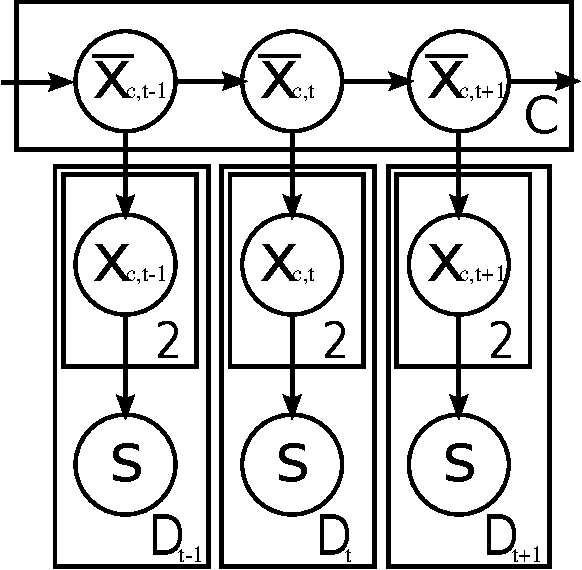
\includegraphics[width=0.26\textwidth]{chapter_foreign_relations/figures/countries_gm_no_text.pdf} \\ (A) \vspace{50pt} \\
      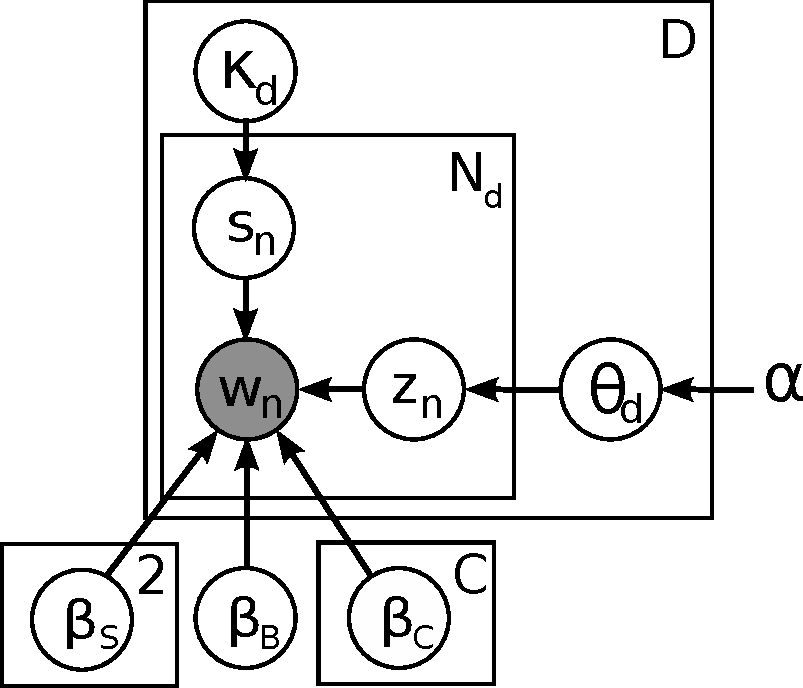
\includegraphics[width=0.35\textwidth]{chapter_foreign_relations/figures/fr_lda_gm.pdf} \\ (B) \\
    \end{tabular}
    &
    \begin{tabular}{c}
    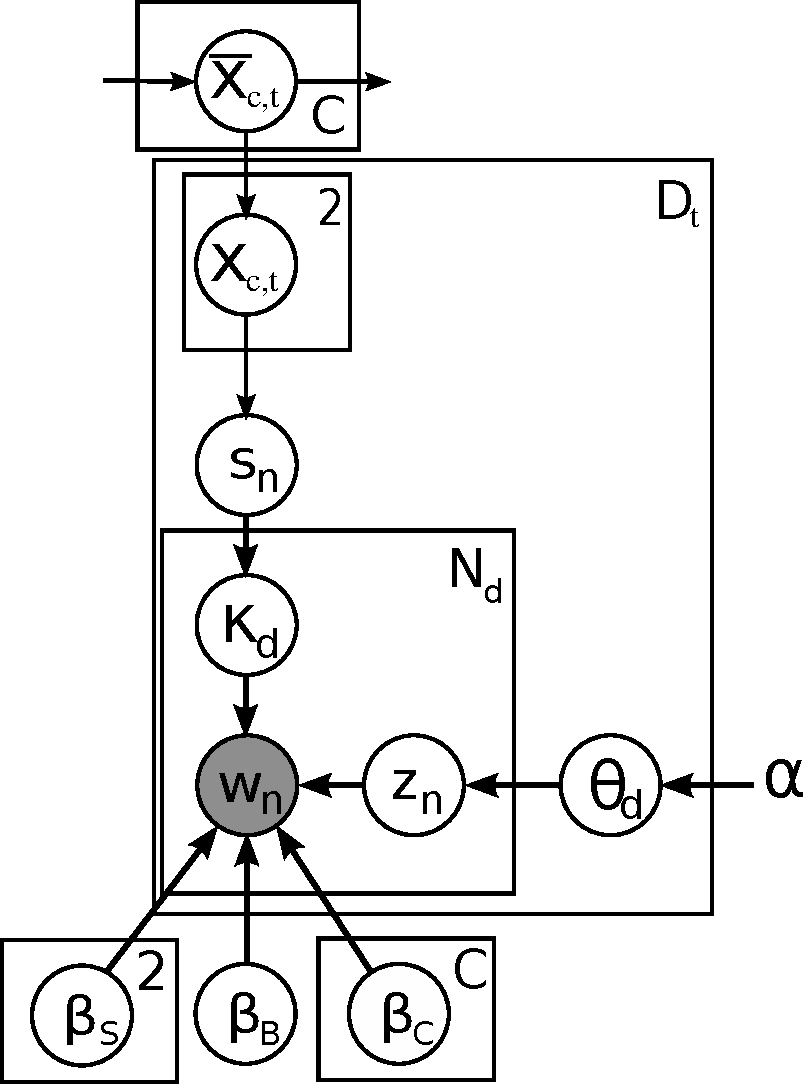
\includegraphics[width=0.35\textwidth]{chapter_foreign_relations/figures/countries_gm_unsupervised_all.pdf} \\ (C) \\
    \end{tabular}
  \end{tabular}
  \caption{The dynamic sentiment model (A), a binary mask
    mixed-membership language model (B), and the full unsupervised
    foreign relations model (C) (which is a combination of (A) and
    (C).  In (B) and (C), we assign each country its own topic
    $\beta_{C,\cdot}$.  Interactions between countries are
    characterized by sentiment $s_d$, which is reflected in the
    sentiment topic $\beta_{S,\kappa_d}$.  The background topic
    $\beta_B$ is provided to ``soak up'' background noise.}
  \label{fig:dynamic_dyadic_chain}
  \label{fig:binary_relational_language_model}
  \label{fig:dynamic_dyadic_chain_binary_relational_language_model}
\end{figure}

\subsection{Inference}
As before, we only observe a collection $\{ (\bm w_d, c_{d,1},
c_{d,2}) \}_{d \in D}$ of interactions between countries.  Each of
these interactions takes the form of a vector of wordcounts $\bm w_d$
and a pair of countries interacting.  To perform an empirical analysis
with this model, we must estimate the latent positions of countries
and the latent topics associated with documents.  These are described
by the hidden random variables $\bar x_c, \theta$, and $\beta$.
We accomplish this with posterior inference, which will provide us
with an estimate of the distribution $p(\bar x_c, \theta, \beta |
\{ (\bm w_d, c_{d,1}, c_{d,2}) \}_{d \in D})$.

We fit this model with \emph{maximum a posteriori} (MAP) inference,
which has the benefit of a simpler derivation than variational
inference.  As the reader may recall, the MAP estimate is
\begin{align}
  \hat x_c, \hat \theta, \hat \beta
  = & \arg \max_{\bar x_c, \theta, \beta} p(\bar x_c, \theta, \beta | \{ (\bm w_d, c_{d,1}, c_{d,2}) \}_{d \in D}) \nonumber \\
  = & \arg \max_{\bar x_c, \theta, \beta} p(\bar x_c, \theta, \beta, \{ (\bm w_d, c_{d,1}, c_{d,2}) \}_{d \in D}). \label{equation:fr_unsupervised_map_likelihood}
\end{align}

Deriving the algorithm for MAP estimation requires expanding the full
likelihood objective, lower-bounding this objective, and maximixing
the lower bound with respect to the parameters.  We have designed the
model in such a way that updates can be performed by a combination of
exact coordinate ascent on each parameter (or its expectation), with
the exception of countries' mean position $\hat x_{c_{d,1}, c_{d,2}}$
during interactions.

The lower bound on the likelihood uses the expectations
$\expect{\kappa_d}$ and $\expect{z_n}$.  This means that each
interaction is manifested as a mixture $\expect{\kappa_d}$ of
sentiment, and the observed words are treated as mixtures $\expect{\bm
  z_d}$ of topics.  We estimate countries' mean positions $\bar \hat
x$ using a Kalman filter \citep{kalman:1960} as in the last section.
This inference step is exactly as in the last section.


\paragraph{Countries' per-interaction positions $x_{c_{d,1}, c_{d,2}}$.}
As in the last section, we infer countries' positions during an
interaction by gradient ascent on the objective with respect to their
positions $x_{c_{d,1}, c_{d,2}}$.

\paragraph{Estimating topics $\beta_{C, \cdot}, \beta_{S, \cdot}$, and $\beta_{B}$.}
The update for topics is similar to that in LDA.  In both cases, we
aggregate the sufficient statistics and normalize during an M-step.
We also use Laplace smoothing by adding pseudo counts of
$0.1$ to these statistics.

\paragraph{Estimating $\expect{\kappa}$ and $\expect{z_n}$.}
During inference, we compute the expectations $\expect{\kappa_d}$ and
$\expect{z_n}$, to perform EM.  The goal of performing EM is to optimize the bound
\begin{align}
  \log p(\bm w_d | \bm \beta, s_d)
  & \ge \log \expectq{ \frac{q(\kappa_d, \bm z_d)}{q(\kappa_d, \bm z_d)} p(\bm w_d | \bm \kappa_d, \bm z_d, \bm \beta, s_d) } \\
%  & = \expectq{ \frac{ q(\kappa_d) }{ q(\kappa_d) } \log \frac{ p(\bm w_d | \bm \kappa_d, \bm z_d) }{ q(\kappa_d) } } \\
  & \ge \expectq{ q(\kappa_d, \bm z_d) \log \frac{p(\bm w_d | \bm
      \kappa_d, \bm z_d, \bm \beta, s_d)}{q(\kappa_d, \bm z_d)} } \\
  & = \expectq{ p(\bm w_d | \bm \kappa_d, \bm z_d, \bm \beta, s_d)}
  - H(q(\kappa_d, \bm z_d))
\label{eq:fr_em_motivation}
\end{align}
on the likelihood of documents, where we specify $q(\bm \kappa_d, \bm
z_d)$ to be the factorized distribution $q(\bm \kappa_d) q(\bm z_d)$
and write the expectations $q(\bm \kappa_{d} = 1) = \expectq{\bm
  \kappa_d}$, $q(\bm z_{dn}=1) = \expectq{(\bm z_{d,n})}$.

As an aside, note the similarity between \myeq{fr_em_motivation} and
the variational objective (\myeq{traditional_variational_objective}).
MAP inference using EM can be interpreted as variational inference, in
which we use point estimates for many of the random variables and
distributions to represent the remaining variables.

Letting $S_0$ and $S_1$ index the sentiment word-topic distributions,
and letting $S$ index the sentiment topic in the topic indicators $z$,
and recalling that the indicator $z_n$ describes word $w_n$, this
update is:
\begin{align}
  \kappa_{d,0} & \propto \sum_{n=1}^{N_d} \beta_{S_0,w_n} \expect{z_{n,S}} \nonumber \\
  \kappa_{d,1} & \propto \exp(s_d) \sum_{n=1}^{N_d} \beta_{S_1,w_n} \expect{z_{n,S}} \nonumber \\
  \expect{\kappa_{d,i}} & = \frac{\kappa_{d,m}} { \sum_k \kappa_{d,m} } \nonumber \\
\end{align}

The update for $\expect{z_{n}}$ is similar.  Again letting $S (S_0,
S_1)$ refer to the sentiment topic indices, and describing the
remaining indices with $C_1, C_2, B$, we have:
\begin{align}
  z_{n,S} & \propto \expect{\theta_{S}} \left( \beta_{S_0,w_n} \expect{\kappa_{d_z, 0}} + \beta_{S_1,w_n} \expect{\kappa_{d_z, 1}} \right) \nonumber \\
  z_{n,k_{c1}} & \propto \expect{\theta_{C_1}} \beta_{C_1,w_n}  \nonumber \\
  z_{n,k_{c2}} & \propto \expect{\theta_{C_2}} \beta_{C_2,w_n} \nonumber \\
  z_{n,k_{b}} & \propto \expect{\theta_{B}} \beta_{B,w_n} \nonumber \\
  \expect{z_{n,i}} & = \frac{ z_{n,i}} { \sum_k z_{n,k} } \label{equation:fr_e_z}
\end{align}

The update for $\expect{\theta_k}$ is similar to $\kappa_{dk}$, but we use sufficient statistics from all documents:
\begin{align}
  \theta_{k} & \propto \sum_{d=1}^D \sum_{n=1}^{N_d} \expect{z_{n,k}} \nonumber \\
  \expect{\theta_{k}} & = \frac{\theta_{k}} { \sum_m \theta_{m} } \nonumber \\
\end{align}

\subsection{Empirical analysis}
In this section we perform a very cursory empirical discussion of this
model. For this analysis, we used the same \emph{New York Times} (NYT)
articles described in the last section.  The dimension of the latent
space was $p=2$.

% \paragraph{XXX.}  The xxx corpus included xxxx articles from which we
% isolated xxxx paragraphs which mentioned exactly two countries. There
% were xxx distinct countries mentioned in these paragraphs.  We defined
% a vocabulary of size xxxx by removing words appearing in fewer than
% xxx\% of documents or more than xxx\% of documents.  We split these
% paragraphs into a set of xxxx training documents and xxxx test documents.

